% explain ML basics
Machine learning involves the use of computer algorithms to make decisions based on training data. Generally, this falls into categorizing input data (classification) or determining a mathetmatical function to determine a continuous output given an input (regression). Popular classification examples include recognizing handwritten digits (MNIST) as well as determining whether an image contains a cat or a dog. (REF) An example of a regression problem is determining the temperature given a set of input features (humidity, latitude, longitude, date, etc.).

Problems where training data contain input data vectors as well as the correct output vectors (targets) are known as supervised learning problems. Training a model to denoise audio where noise was introduced to the clean audio would be a supervised learning problem. On the other hand, training a model to denoise audio where the underlying clean signal is not known is an unsupervised learning problem. Different loss functions and neural network architectures can be exploited to accomplish denoising without the clean data.

For the purposes of this thesis, we use machine learning to determine an underlying nonlinear function that removes noise from time slices of audio (i.e. regression). These slices can then be pieced back together through overlap-add resynthesis. To clarify, this is a general linear model that maps an input noisy audio vector $y[n]=x[n]+N[n]$ to $\tilde{x}[n]$, a target denoised audio vector, where $x[n]$ is the underlying clean signal and $N[n]$ is the additive background noise.

\subsubsection{Regression}
A classical regression technique is linear regression, where one or more independent variables $x_{i}$ are used to determine a scalar dependent variable $y$. The case of a single independent variable $x$ is known as simple linear regression. On the other hand, the case of estimating  A canonical example would be estimating a sine wave $x[n]$ given noisy samples


\subsubsection{Overfitting and Curse of Dimensionality}


\subsubsection{Loss functions and Regularization}


\subsubsection{Gradient Stuff?}


% Machine learning in general encompasses all tasks where we utilize data to
% make some kind of descision. Classical examples include handwritten digit
% recognition, and flower species classification based on sepal width and petal
% length. As rough mathematical example, consider a sample of N pairs of
% examples drawn from larger population $\mathcal{P}$:
% \begin{gather}
% \mathcal{D} = \left\{(x_i, y_i) \colon i = 1,2, \dots, N \right\}\\
% \mathcal{D} \subset \mathcal{P}
% \end{gather}

% Our machine learning task may be to find some function $f(x)$ that estimates
% $y$ for any $(x,y)$ sample drawn from the population at large. To learn the
% function we might setup a loss function $l(y,\hat{y})$ to quantify how well
% our model performs on our sample $\mathcal{D}$. As a general rule, the loss function
% satisfies the following limit:
% \begin{equation}
% \lim\limits_{\hat{y_i}\to y_i} l(y_i, \hat{y_i}) = 0
% \end{equation}
% In other words our goal is to find some $f(x)$ that minimizes the loss
% function $l(y, \hat{y})$ for all $(x_i, y_i)$ pairs in $\mathcal{D}$. This
% type of task is referred to as supervised learning, because we have a domain
% of inputs and a specified codomain of targets; there are other applications
% with unknown targets, these tasks are referred to as unsupervised learning
% tasks. With a few extra constraints we are able use a number of techniques to
% accomplish this supervised learning goal.

% \subsubsection{Differentiable parametric modeling}
% Let us restrict our study of functions $f$ specifically to functions that are
% differentiable and parametric in form, so from now on we refer to $f(x \mid
% \theta)$ where $\theta$ refers to the function's set of parameters. Using these
% new terms our goal is to find some $\hat{\theta}$ that satisfies the following:
% \begin{equation}
% \hat{\theta} = \argmin\limits_\theta l(y, f(x \mid \theta)), \; \forall x, y
% \end{equation}

% For any problem of this type we would like to calculate gradient of $l$ with
% respect to each $\theta_i$, set them all to zero and solve for each $\theta_i$:
% \begin{equation}
% \frac{\partial l(x, f(x \mid \theta))}{\partial \theta_i} = 0, \; \forall i
% \end{equation}

% However this is not always possible analytically because without convexity
% constraints we are not able to guarantee the existence of a unique minimum in
% the loss function.

% In lieu of an analytic solution we can use a numerical optimization approach, and
% jointly optimize the $\theta_i$'s via a gradient descent algorithm. For
% example we could use this update rule, which we refer to as steepest descent:
% \begin{equation}
% \theta_i \leftarrow \theta_i - \eta \frac{\partial l(x, f(x \mid \theta))}{\partial \theta_i}
% \end{equation}

% where $\eta$ is a the learning rate parameter, which controls how large our
% steps are towards the minimum.

% \subsubsection{Basis expansions}
% Let us consider our first supervised learning example. Consider a noisy
% sine-wave consisting of $k$ samples:
% \begin{equation}
% \mathbf{y} = \sin \mathbf{x} + \mathbf{n}, \; \mathbf{y}, \mathbf{x}, \mathbf{n} \in \mathbb{R}^k
% \end{equation}
% We would like to find some $f(\mathbf{x} \mid \theta)$ that produces an estimate $\hat{\mathbf{y}}$. Let us consider the following functional form for $f$:
% \begin{equation}
% f(\mathbf{x}) = m\mathbf{x} + b,\; m,b \in \mathbb{R}
% \end{equation}
% Or we can rewrite this as a matrix multiplication by padding x in with a ones
% vector to create a $2 \times k$ matrix we refer to as $\Phi$, and combining
% $m$ and $b$ into a vector $\mathbf{w}$:
% \begin{equation}
% \hat{\mathbf{y}} = \mathbf{w}^T\Phi
% \end{equation}
% We are able to compute $\hat{m}$ and $\hat{b}$ analytically, with a mean
% squared error loss function:
% \begin{equation}
% l(\mathbf{y}, \hat{\mathbf{y}}) = \frac{1}{2}\sum\limits_{i=1}^k(\hat{y_i} - y_i)^2
% \end{equation}
% Now let's substitute our model in for $\hat{y}$ and set the gradient to zero:
% \begin{equation}
% \frac{\partial l(\mathbf{y}, \hat{\mathbf{y}})}{\partial \mathbf{w}} \left(\frac{1}{2}\sum\limits_{i=1}^k(\mathbf{w}^T\Phi - y_i)^2\right) = 0
% \end{equation}
% Carrying out the derivative we see:
% \begin{equation}
% \frac{1}{2}\sum\limits_{i=1}^k(\mathbf{w}^T\Phi - \mathbf{y})\Phi^T = 0
% \end{equation}
% \begin{figure}
% \centering
% 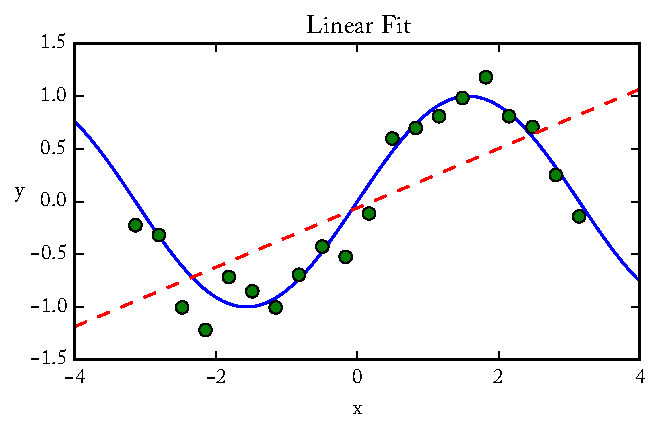
\includegraphics[width=0.5\textwidth]{figures/sinewave_lin.pdf}
% \caption[Linear regression of a noisy sine-wave]{Linear
% regression of a noisy sine-wave.}
% \label{expand}
% \end{figure}
% \begin{figure}
% \centering
% 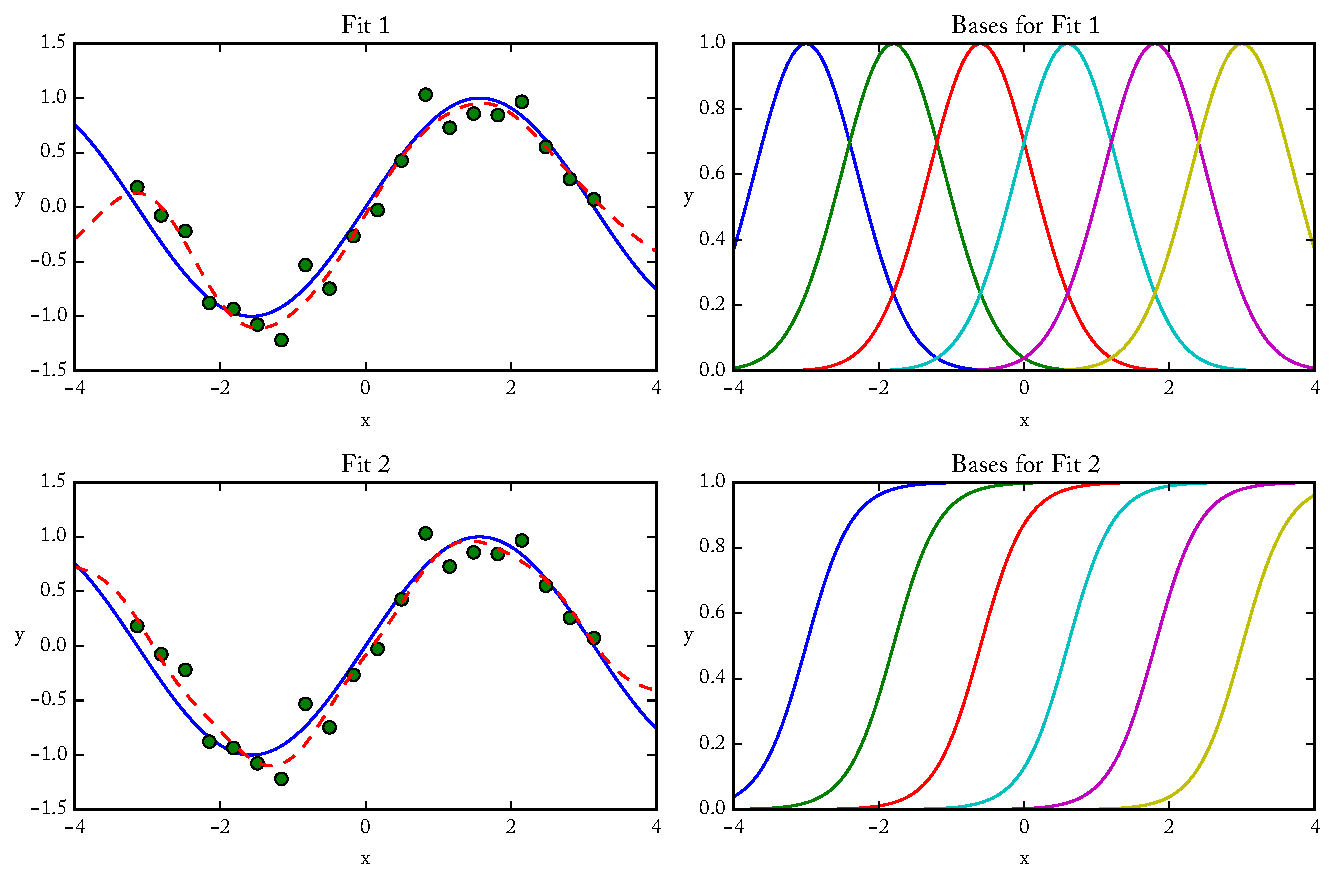
\includegraphics[width=\textwidth]{figures/sinewave.pdf}
% \caption[Linear regression of a noisy sine-wave with basis expansion]{Linear
% regression of a noisy sine-wave with basis expansion}
% \label{expand}
% \end{figure}
% \subsubsection{Kernel methods}
% \subsubsection{Curse of dimensionality}
% \subsubsection{Over-fitting}
% \begin{figure}
% \centering
% 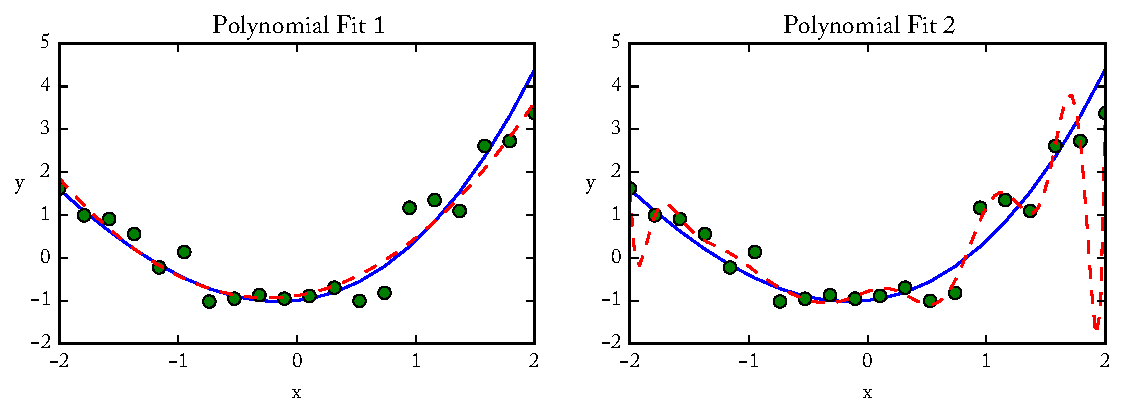
\includegraphics[width=\textwidth]{figures/polyfit.pdf}
% \caption[Polynomial Fit]{Polynomial Fit}
% \label{overfit}
% \end{figure}
